% Combined version of Rowan's first draft, which is kept unchanged in
% usv-intervention/solution/rowan/docs/3/3_Solution_Jake_Rowan.tex.
% It adds Jake's linear-regression findings (jake/linear-reg/) as Section 3.2 and lines the
% notation up with Milestones 1 and 2. Passages added or reworded here are marked "% [Claude]";
% the rest is as in Rowan's file.
%
% PAGE LIMIT (exactly 2 pages). The version without keywords compiled to 2 pages with about 3 lines to spare.
%   Keywords were added after that, and this version has not been compiled yet. To make room, four lines were
%   taken out of the first column of page 1 (the "In words" sentence, and tighter wording in the abstract and
%   introduction), so that everything from Section 3.1 onwards stays where it was.
%   If it runs onto a 3rd page: shorten the abstract or the introduction by one more line. The first column of
%   page 1 is what matters; cutting text on page 2 will not help as much.
%   If there is room left at the end: ADD-BACK 2 and ADD-BACK 3 (one line each) fit there.
\documentclass[sigconf]{acmart}
% Cleaning
\pagestyle{fancy} % removes running headers
\settopmatter{printacmref=false} % Removes citation information below abstract
\renewcommand\footnotetextcopyrightpermission[1]{} % removes footnote with conference information in first column
\pagestyle{plain} % removes running headers
\fancyhead{}
\settopmatter{printacmref=false, printfolios=false}
% Copyright
\setcopyright{none}
\settopmatter{printacmref=false} % Removes citation information below abstract
\acmDOI{}

\usepackage{booktabs} % For formal tables
\usepackage{url}
\usepackage{algorithm}
\usepackage[noend]{algpseudocode}
\algtext*{EndWhile}% Remove "end while" text
\algtext*{EndIf}% Remove "end if" text
\algtext*{EndFor}% Remove "end for" text

\setlength{\parskip}{0pt}
\setlength{\parsep}{0pt}
\setlength{\headsep}{0pt}
\setlength{\topskip}{0pt}
\setlength{\topmargin}{0pt}
\setlength{\topsep}{0pt}
\setlength{\partopsep}{0pt}
\usepackage{mdwlist}
\usepackage{amsmath}
\usepackage{tikz}
\usetikzlibrary{positioning,arrows.meta}

\begin{document}
% [Claude] title shortened to one line, in the pattern of the Milestone 1 and 2 titles.
% Rowan's original: Learning USV Drift from Telemetry: Linear, LSTM and Transformer Models
\title{Predicting One-Hour Drift for a Station-Keeping USV}
\author{Jake Cushway}
\affiliation{
  \institution{University of Victoria}
  \city{Victoria}
  \country{Canada}
}
\email{jakecush1@uvic.ca}

\author{Rowan Hall}
\affiliation{
  \institution{University of Victoria}
  \city{Victoria}
  \country{Canada}
}
\email{rowanhall@uvic.ca}

\begin{abstract}
% [Claude] one sentence added on the linear fits; repo path updated to the renamed folder; wording tightened by one
% line to make room for the keywords ("define the task as regression" is now covered by the keyword list)
Between course corrections, the DataXplorer\texttrademark{} USV drifts with its motor off, and a pilot must step in before wind and current carry it out of its 10~nm station. We predict where it will be in one hour, using only its last hour of GPS track and wind. Linear fits show wind speed explains under 15\% of drift, and past drift most of it. We compare four models (persistence, linear regression, LSTM, transformer) on an unseen deployment. Code: \url{https://github.com/jakecush1/autonomous-pilot-ML} (\texttt{usv-intervention/solution}).\footnote{AI use (Guideline D): the code and a first draft of this paper were generated with Claude (Anthropic) and reviewed, run and edited by the authors.}
\end{abstract}

% [Claude] Rowan's keywords, with "Uncrewed surface vehicle" shortened to "USV" so that they fit on one line.
% Rowan's original: Uncrewed surface vehicle, drift prediction, time series regression, LSTM, transformer
\keywords{USV, drift prediction, time series regression, LSTM, transformer}
\maketitle
\pagestyle{empty}

\section{Introduction}\label{sec:intro}
% [Claude] reworded to link back to Milestones 1 and 2; contribution list now includes the analysis of Section 3.2;
% wording tightened by one line to make room for the keywords
The Open Ocean Robotics DataXplorer replaces a retired NOAA weather buoy and must stay within 10~nm of the buoy's position. It mostly drifts with the motor off, and a pilot watches it 24/7 although a correction is needed only every 2--3 hours. Milestones~1 and~2 set out to predict \emph{when} the pilot must act. The first step is predicting \emph{where} the drifting vessel is going: a position predicted an hour ahead can be checked against the 10~nm limit to alert the pilot early. Unlike drift models built on physics and weather forecasts~\cite{dugan2024drifting,song2024drift}, we learn drift from the vessel's own telemetry. We contribute a formal task definition, an analysis of what drives drift, a leak-free data pipeline, and a comparison of four models.

\section{Problem Definition}\label{sec:problem}
% [Claude] removed to make room for the keywords (2 lines); the abstract says the same thing. Rowan's sentence:
% \emph{In words: given the last hour of a drifting vessel's track and wind, predict how far it will move east and north in the next hour.}
%
% [Claude] the state is written as in Milestone 1 (position, wind speed, wind direction) plus motor power.
% The drift function is now g, because Milestone 1 already uses f for the intervention decision and R for the 10 nm limit.
A deployment is a sequence of 1-minute telemetry records $\mathcal{S}=\{s_\tau\}_{\tau=1}^{T}$. As in Milestone~1, $s_\tau=(p_\tau,v_\tau,\theta_\tau,m_\tau)$ holds position (latitude, longitude), wind speed (kn) and the direction the wind blows \emph{from}, plus motor power (W). The vessel is \emph{drifting} at minute $\tau$ if $m_\tau=0$. Let $\mathbf{p}_\tau\in\mathbb{R}^2$ be its position in metres east and north of the station $p_0$ (\S\ref{sec:repr}). For a time $t$ at which the vessel has drifted for the past $H$ minutes, our solution is a function
\begin{equation}\label{eq:g}
g:\mathbb{R}^{H\times 4}\rightarrow\mathbb{R}^{2},\qquad \hat{\mathbf{y}}_t=g(\mathbf{X}_t)\approx\mathbf{y}_t=\mathbf{p}_{t+H}-\mathbf{p}_t,
\end{equation}
where $\mathbf{X}_t$ describes the past $H$ minutes (4 numbers per minute) and $\mathbf{y}_t$ is the movement over the next $H$ minutes, assuming the motor stays off. The predicted position $\hat{\mathbf{p}}_{t+H}=\mathbf{p}_t+\hat{\mathbf{y}}_t$ can then feed the decision $f$ of Milestone~1, which checks it against the limit $R=10$~nm. The output is a distance, not a category, so this is regression, not classification. We use $H=60$ (\S\ref{sec:explore}).

\section{Proposed Approach}\label{sec:approach}
Figure~\ref{fig:pipeline} shows the pipeline and Algorithm~\ref{alg:drift} gives the pseudo-code.

\subsection{Representation}\label{sec:repr}
% [Claude] station written as p_0 (Milestone 1); Earth radius renamed r, since R is the 10 nm limit
\textbf{Position.} Positions $(\phi_\tau,\lambda_\tau)$ are converted to metres from the station $p_0=(\phi_0,\lambda_0)$, so that distances and movements are meaningful: $\mathbf{p}_\tau=r\,\big((\lambda_\tau-\lambda_0)\cos\phi_0,\;\phi_\tau-\phi_0\big)$, with Earth radius $r=6371$\,km and angles in radians. This flat-earth approximation is off by less than 0.3\% within 10~nm.
\textbf{Wind.} The wind blowing \emph{from} direction $\theta$ pushes the vessel the opposite way, so we use the push vector $\mathbf{w}_\tau=-v_\tau(\sin\theta_\tau,\cos\theta_\tau)$ (east, north).
% ADD-BACK 3 (1 line), goes at the end of the Wind sentence above:
% Using sine and cosine also avoids the jump from 359° to 0°.
\textbf{Input window.} For each minute we keep its movement $\Delta\mathbf{p}_\tau=\mathbf{p}_\tau-\mathbf{p}_{\tau-1}$ and the wind push, giving
$\mathbf{X}_t=[\,(\Delta\mathbf{p}_\tau,\mathbf{w}_\tau)\,]_{\tau=t-H+1}^{t}$, a table of 60 rows by 4 columns.

% [Claude] new subsection with Jake's findings. Sources: jake/linear-reg/drift-vs-wind/notes.md
% (wind-speed fit, window sweep) and jake/linear-reg/drift-prediction/notes.md (past drift + wind,
% R^2 by H). Every number was re-run from his two scripts on the five deployments and matches.
\subsection{What Drives the Drift?}\label{sec:explore}
On the motor-off data, \textbf{wind speed alone} explains little: a linear fit, drift speed $=0.72\,v+8.1$ (m/min, $v$ in kn), has $R^2\le0.15$ for speed measured over any window from 1 to 60 minutes, best at 10 (shorter adds GPS noise, longer blurs changes). The slope is 2.3\% of the wind speed, and the 0.26\,kn of drift left with no wind shows that current matters at least as much as wind. \textbf{Adding wind direction and the past $H$ minutes of drift} raises $R^2$ to 0.83 at $H=60$: the next hour is 0.84--0.92 of the last, turned slightly clockwise. Past drift captures current and tide without measuring them, so every model takes it as input. The fit weakens as $H$ grows ($R^2=0.93$, 0.91, 0.83 at $H=1$, 30, 60), since wind and current have longer to change, but a pilot needs an hour of warning, so we keep $H=60$. These $R^2$ are on training data; \S\ref{sec:impl} tests on an unseen deployment.

% OPTIONAL TABLE (about 7 lines; only fits if something else of that size goes, e.g. the worked example).
% To use it, uncomment it and point to it from the paragraph above with Table~\ref{tab:explore}.
% The H = 5 and H = 10 values in the second row are from a re-run of future.py, not from Jake's notes.
% \begin{table}[t]
% \caption{Linear fits: training $R^2$ by window/horizon (min).}
% \label{tab:explore}
% \footnotesize
% \begin{tabular}{@{}lccccc@{}}
% \toprule
% Inputs $\rightarrow$ target & 1 & 5 & 10 & 30 & 60 \\
% \midrule
% Wind speed $\rightarrow$ drift speed & 0.125 & 0.144 & 0.145 & 0.127 & 0.104 \\
% Past drift, wind $\rightarrow$ movement & 0.931 & 0.959 & 0.954 & 0.912 & 0.830 \\
% \bottomrule
% \end{tabular}
% \end{table}

\subsection{Cleaning and Splitting the Data}\label{sec:data}
Gaps of up to 5 missing minutes are filled by linear interpolation. A minute is \emph{valid} if the motor is off, no value is missing, and the vessel moved less than 93\,m (about 3\,kn; faster means it was being towed, not drifting). A time $t$ becomes a training sample $(\mathbf{X}_t,\mathbf{y}_t)$ only if all 120 minutes from $t-59$ to $t+60$ are valid, so neither the input nor the answer includes motor use. Five deployments (Apr--Oct 2026, 85{,}915 minutes) give 23{,}319 samples.

Samples one minute apart share 59 of their 60 input minutes, so a random train/test split would put near-copies of test samples in training. We therefore split by whole deployment: \textbf{train} (Apr, May--Jun, Aug; 16{,}471 samples), \textbf{validation} (Oct 3--13; 2{,}289), used only to decide when to stop training, and \textbf{test} (Oct 16--23; 4{,}559), never used for any choice. Inputs and targets are rescaled to mean 0 and standard deviation 1 using training data only.
% ADD-BACK 2 (1 line), goes at the end of the paragraph above:
% A sixth deployment (Nov 2--9) is held out for Milestone~4.

\subsection{Models}
% [Claude] f -> g; linear regression tied to Section 3.2; model sizes moved here from the
% hyperparameter table, which is removed to make room for Section 3.2
Each model is a different way to compute $g$ in Eq.~\ref{eq:g}.
\textbf{(1) Persistence} (no training): the next hour repeats the last, $\hat{\mathbf{y}}_t=\sum_{\tau}\Delta\mathbf{p}_\tau$. Current and tide change slowly, so this is a strong bar to beat.
\textbf{(2) Linear regression}: $\hat{\mathbf{y}}_t=\mathbf{A}\,\mathbf{z}_t+\mathbf{c}$, the fit of \S\ref{sec:explore} plus mean wind: $\mathbf{z}_t$ summarises the window in 6 numbers (past-hour movement, current wind push, mean wind push over the hour) and $\mathbf{A}\in\mathbb{R}^{2\times6}$, $\mathbf{c}$ are fitted by least squares. Its weights can be read directly.
\textbf{(3) LSTM}~\cite{hochreiter1997lstm} (2 layers, 64 hidden units, dropout 0.2): reads the 60 rows of $\mathbf{X}_t$ one minute at a time, updating a memory vector $\mathbf{h}$; the final $\mathbf{h}_t$ is mapped to $\hat{\mathbf{y}}_t=\mathbf{W}\mathbf{h}_t+\mathbf{b}$. Unlike the 6-number summary, it can see whether the drift is turning or slowing down.
\textbf{(4) Transformer}~\cite{vaswani2017attention} (2 layers, width 64, 4 heads, feed-forward 256, dropout 0.1): each minute becomes a 64-number vector plus a code for its position in time, $\mathbf{e}_\tau=\mathbf{W}_e\mathbf{x}_\tau+\mathrm{PE}(\tau)$. Self-attention layers let every minute compare itself with every other; the outputs are averaged over the hour and mapped to $\hat{\mathbf{y}}_t$. A more complex model is only worth using if it beats the simpler one on unseen data.

\subsection{Training, Inference and Scoring}
% [Claude] training settings moved here from the hyperparameter table
The LSTM and transformer minimise mean squared error with Adam~\cite{kingma2015adam} (learning rate $10^{-3}$, batch 256, gradient clip 1.0, seed 0). After each pass over the training data (epoch) we keep the weights with the lowest validation loss and stop after 10 epochs without improvement, or after 80. This matters because the 23k overlapping windows hold only about 400 independent hours of drift, and both networks start memorising within a few epochs. These settings are common defaults, not tuned. At inference the output is scaled back to metres and added to $\mathbf{p}_t$.

We score each prediction by its \textbf{endpoint error} $e_t=\|\hat{\mathbf{p}}_{t+H}-\mathbf{p}_{t+H}\|_2$, the distance in metres between predicted and true position. We report the median (a typical miss, robust to GPS glitches) and the 90th percentile (a bad-case miss, usable as a safety radius).

% TRIM 1 (5 lines): the worked example below
\textbf{Worked example.} On Oct 19 at 21:15 (test deployment) the vessel had moved $(774, 555)$\,m east/north in the past hour and was slowing down. Persistence predicts $(774, 555)$\,m again and the LSTM $(460, 353)$\,m; the vessel actually moved $(283, 194)$\,m. The endpoint errors are 609\,m and 238\,m: the LSTM noticed the slowdown.

\begin{algorithm}[t]
\caption{Drift prediction: build data, train, predict}
\label{alg:drift}
\begin{algorithmic}[1]
\Statex\textbf{Input:} deployments $\{\mathcal{S}_k\}$, horizon $H$, model $g_\Theta$
\Statex\textbf{Output:} trained $g_{\Theta^*}$; predicted position $\hat{\mathbf{p}}_{t+H}$
\ForAll{deployments $\mathcal{S}_k$} \Comment{build samples}
\State fill gaps $\leq5$ min; $\mathbf{p}_\tau\gets$ metres from station
\State $\mathbf{w}_\tau\gets-v_\tau(\sin\theta_\tau,\cos\theta_\tau)$ \Comment{wind push}
\State valid$_\tau\gets$ motor off $\land$ no missing $\land\ \|\Delta\mathbf{p}_\tau\|<93$
\ForAll{$t$ where minutes $t{-}H{+}1..t{+}H$ are all valid}
\State add $(\mathbf{X}_t,\ \mathbf{y}_t=\mathbf{p}_{t+H}-\mathbf{p}_t)$ to the split of $\mathcal{S}_k$
\EndFor
\EndFor
\State rescale with train statistics; seed $\gets0$; best $\gets\infty$
\For{epoch $=1..80$} \Comment{train}
\ForAll{mini-batches $B$ of train}
\State $\Theta\gets\mathrm{Adam}\big(\Theta,\nabla_\Theta\tfrac{1}{|B|}\sum_{B}\|g_\Theta(\mathbf{X})-\mathbf{y}\|^2\big)$
\EndFor
\If{val loss $<$ best} best $\gets$ val loss; $\Theta^*\gets\Theta$
\ElsIf{no improvement for 10 epochs} \textbf{break}
\EndIf
\EndFor
\State \Return $\hat{\mathbf{p}}_{t+H}=\mathbf{p}_t+g_{\Theta^*}(\mathbf{X}_t)$ \Comment{predict}
\end{algorithmic}
\end{algorithm}

\begin{figure}[t]
\centering
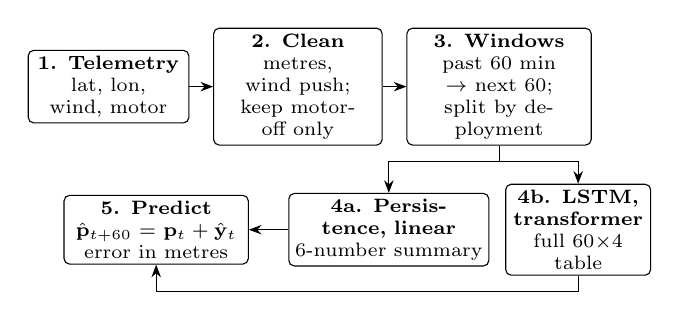
\begin{tikzpicture}[font=\scriptsize, node distance=4mm and 3mm,
  box/.style={draw, rounded corners=2pt, align=center, minimum height=7mm, inner sep=2pt, text width=#1},
  box/.default=20mm,
  arr/.style={-{Stealth[length=1.6mm]}}]
\node[box=19mm] (raw) {\textbf{1. Telemetry}\\lat, lon, wind, motor};
\node[box=20mm, right=of raw] (pre) {\textbf{2. Clean}\\metres, wind push;\\keep motor-off only};
\node[box=22mm, right=of pre] (win) {\textbf{3. Windows}\\past 60 min $\rightarrow$ next 60;\\split by deployment};
\node[box=24mm, below=6mm of win, xshift=-14mm] (lin) {\textbf{4a. Persistence, linear}\\6-number summary};
\node[box=17mm, right=2mm of lin] (seq) {\textbf{4b. LSTM,}\\\textbf{transformer}\\full 60$\times$4 table};
\node[box=22mm, left=5mm of lin] (out) {\textbf{5. Predict}\\$\hat{\mathbf{p}}_{t+60}=\mathbf{p}_t+\hat{\mathbf{y}}_t$\\error in metres};
\draw[arr] (raw) -- (pre);
\draw[arr] (pre) -- (win);
\draw[arr] (win.south) -- ++(0,-2mm) -| (lin.north);
\draw[arr] (win.south) -- ++(0,-2mm) -| (seq.north);
\draw[arr] (lin) -- (out);
\draw[arr] (seq.south) -- ++(0,-2mm) -| (out.south);
\end{tikzpicture}
% [Claude] caption shortened from three lines to two
\caption{Pipeline: each model maps a 60-minute motor-off window of telemetry to the next hour's movement.}
\label{fig:pipeline}
\end{figure}

\section{Implementation}\label{sec:impl}
% [Claude] Jake's scripts added; folder is now solution/
The code is in Python (scikit-learn, PyTorch). The fits of \S\ref{sec:explore} are in \texttt{jake/linear-reg/}; the pipeline is in \texttt{rowan/}, one file per stage, matching Algorithm~\ref{alg:drift}: \texttt{data\_prep.py} (representation, cleaning, split, endpoint error; lines 1--6), \texttt{linear\_reg.py} (persistence, linear regression), \texttt{nn\_models.py} (LSTM, transformer, training loop; lines 7--13) and \texttt{compare.py} (results table, chart). Outputs go to \texttt{outputs/}. The README covers the project, installation, quick start and results; dependencies are pinned in \texttt{requirements.txt} and the data are in the repository. The quick-start script \texttt{quickstart.sh} creates the environment on first use and runs all five steps in order (about 5 minutes on a laptop CPU):
{\footnotesize
\begin{verbatim}
git clone https://github.com/jakecush1/autonomous-pilot-ML
cd autonomous-pilot-ML/usv-intervention/solution/rowan
bash quickstart.sh
\end{verbatim}}
\textbf{Reproducibility.} Seeds are fixed to 0 and the split is fixed by deployment, so the quick start on CPU reproduces Table~\ref{tab:results} exactly (confirmed on three runs).

\begin{table}[t]
% [Claude] caption shortened to one line. Rowan's original: First run: endpoint error after 60 min, unseen test deployment.
\caption{Endpoint error after 60 min, test deployment.}
\label{tab:results}
\footnotesize
\begin{tabular}{@{}lccc@{}}
\toprule
Model & Median (m) & 90th pct. (m) & $R^2$ \\
\midrule
No drift ($\hat{\mathbf{y}}=0$) & 586 & 1515 & 0.00 \\
(1) Persistence & 294 & 570 & 0.80 \\
(2) Linear regression & 318 & 631 & 0.77 \\
(3) LSTM & 247 & 497 & 0.85 \\
(4) Transformer & \textbf{246} & \textbf{477} & \textbf{0.86} \\
\bottomrule
\end{tabular}
\end{table}

% [Claude] the linear-regression sentence now connects the training R^2 of Section 3.2 with the test result
\textbf{First results.} Table~\ref{tab:results} shows the pipeline runs end to end. Persistence already halves the error of assuming no drift. Linear regression's training $R^2$ of 0.83 (\S\ref{sec:explore}) falls to 0.77 on the unseen deployment and does \emph{not} beat persistence, while the LSTM and transformer both do, by about 16\%, and are tied with each other. Milestone~4 will tune the settings, test more seeds and horizons, and turn the prediction into a time until the vessel reaches the boundary~\cite{dugan2024drifting}, toward an intervention probability~\cite{kristensen2022dynamic}.

\bibliographystyle{ACM-Reference-Format}
\bibliography{bibliography.bib}

\end{document}
